\subsection{Umsetzung der GUI im Code}\label{tkintercode}
\paragraph{Klassenstruktur}
Im Vordergrund basiert die Klassenstruktur grundsätzlich auf \gls{gls_ctk} Komponenten (siehe Abb.~\ref{fig:klassenstruktur_frontend}). Dabei gibt es die Klassen \enquote{App}, \enquote{PageFrame}, \enquote{TitleFrame} und \enquote{MeasurementFrame}. Im Programm wird eine \enquote{App} Instanz ausgeführt, welche das Hauptfenster ist. Diese Instanz kann beliebig viele \enquote{PageFrames} enthalten, die wiederum jeweils ein \enquote{TitleFrame} und eine Liste von \enquote{MeasurementFrames} beinhalten. Die \enquote{PageFrames} stellen die einzelnen Seiten dar, welche per Knopfdruck an der \acs{rltanzeige} durchgeblättert werden können. In einem \enquote{TitleFrame} wird immer der Titel der jeweiligen Seite gespeichert \bzw angezeigt. In den \enquote{MeasurementFrame} Instanzen werden hingegen die tatsächlichen Messwerte (Bezeichnung + Wert + Maßeinheit) dargestellt.

\begin{figure}[H]
	\centering
	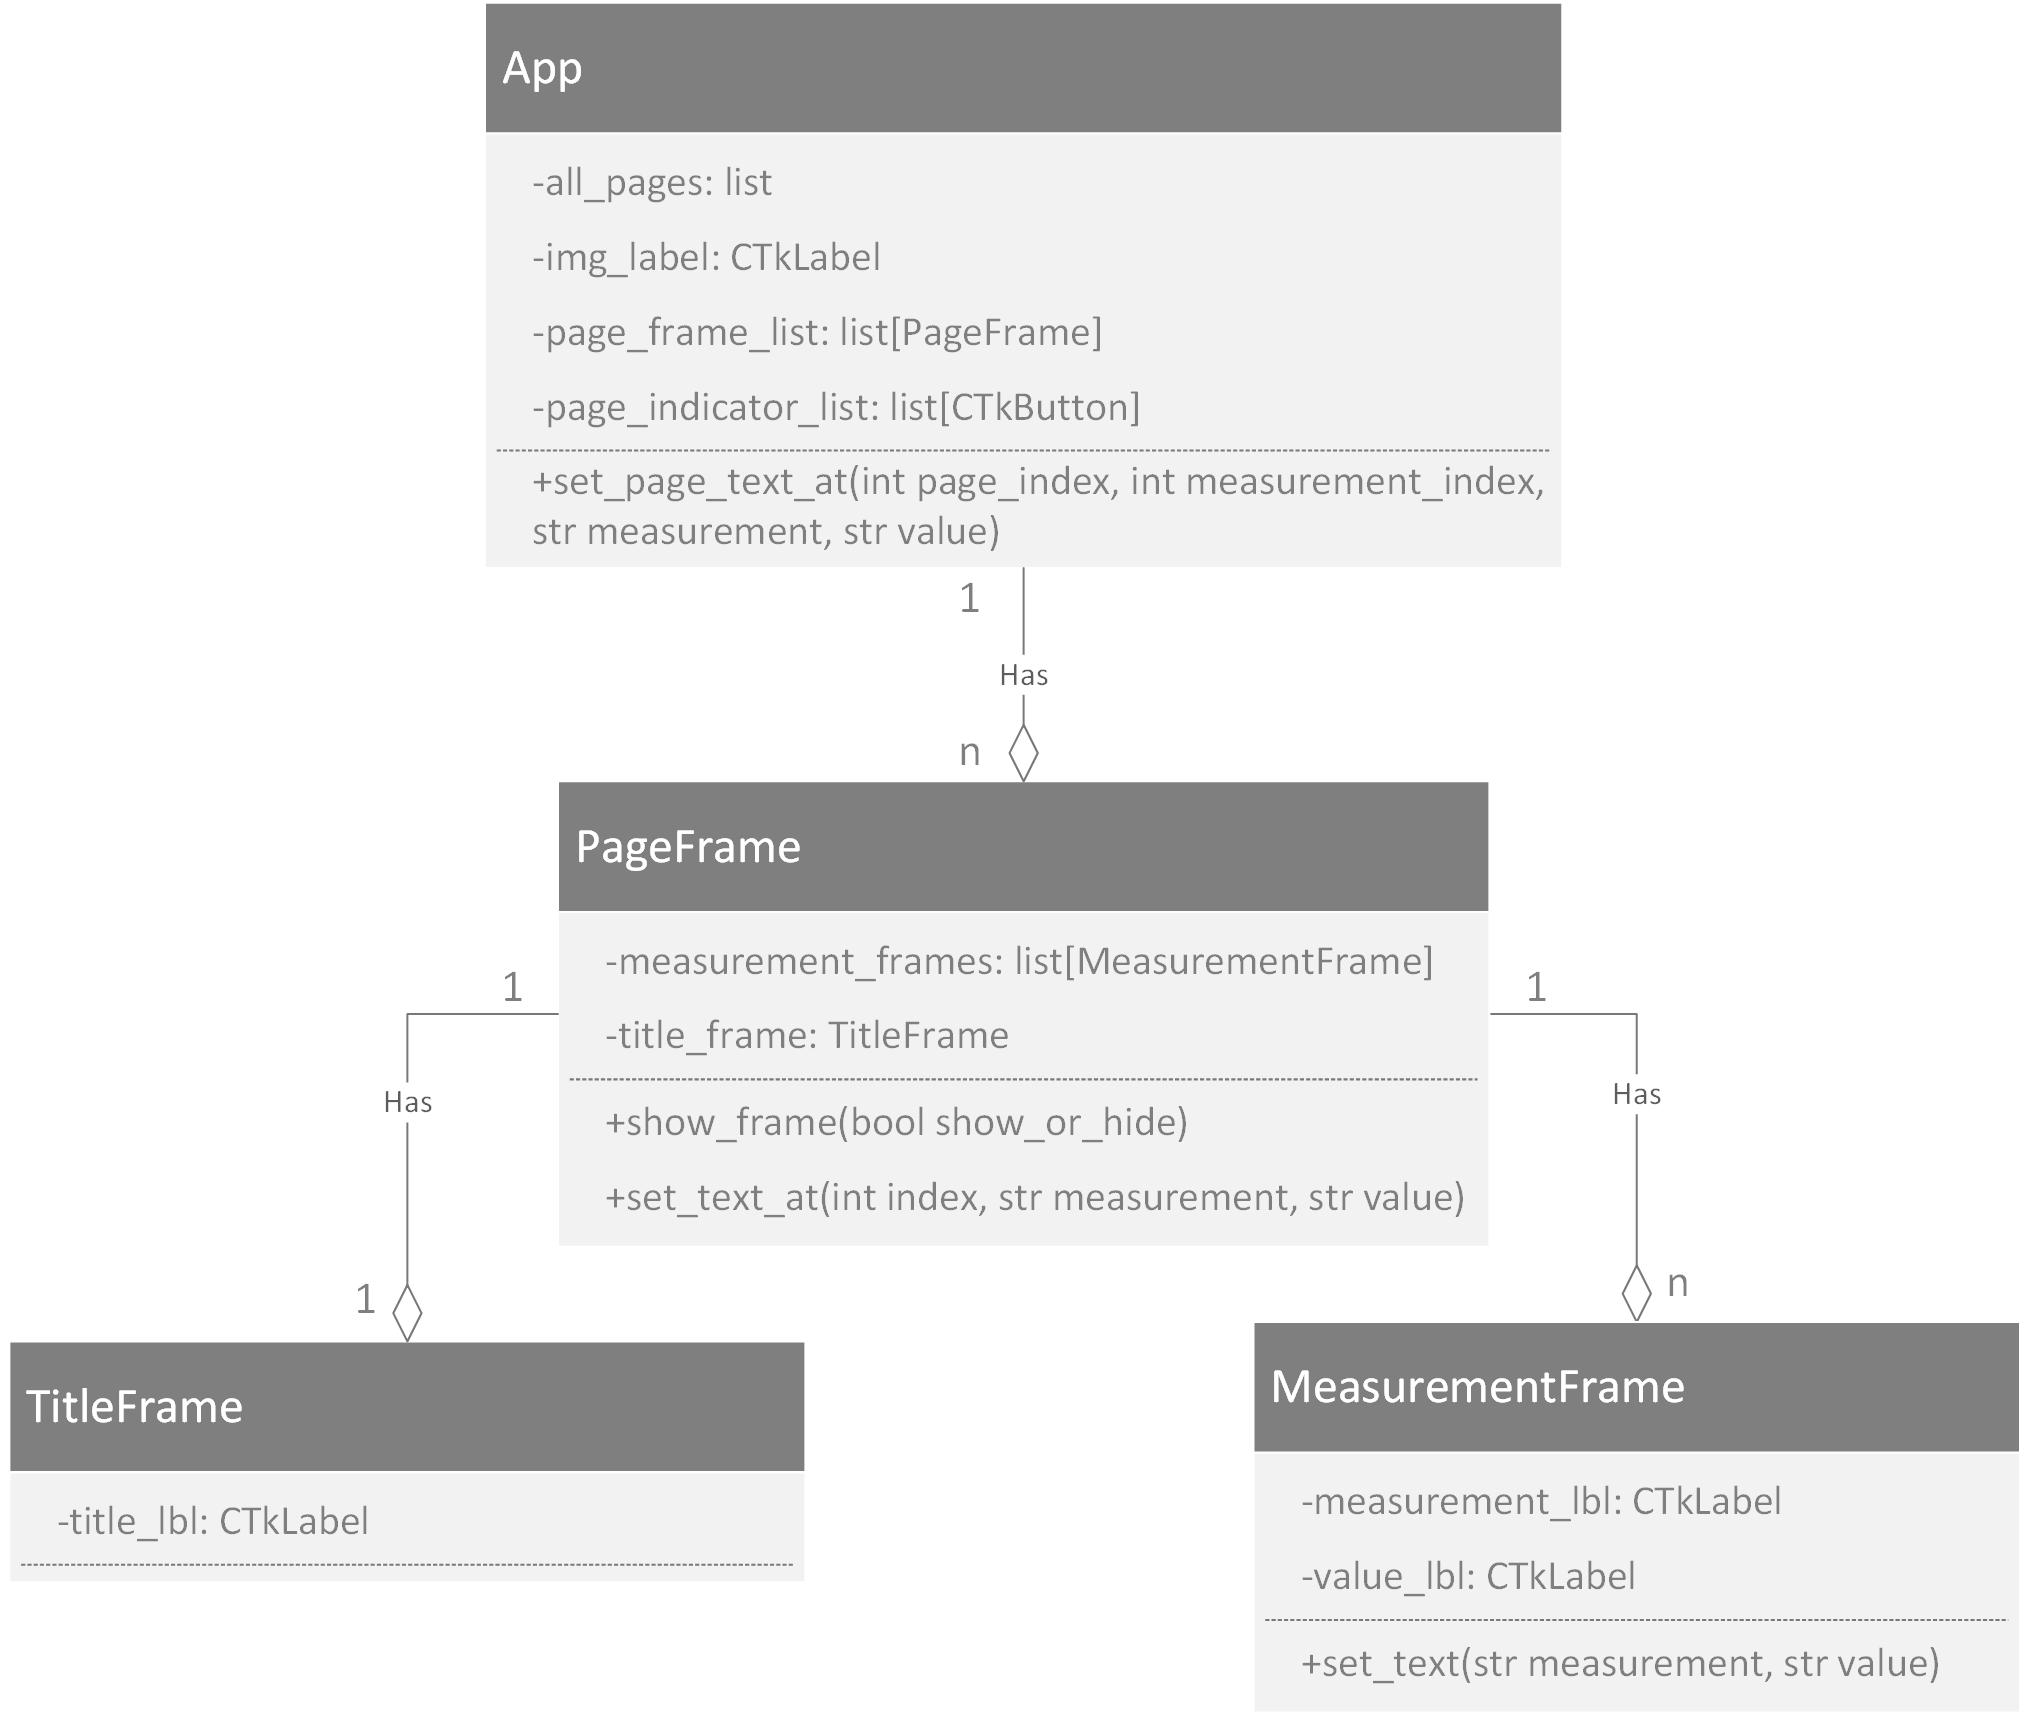
\includegraphics[width=0.95\textwidth]{uml_frontent_class_diagram}
	\caption{UML Diagramm Frontend \label{fig:klassenstruktur_frontend}}
\end{figure}

\paragraph{CustomTkinter Code}
Eine nähere Beschreibung und die Umsetzung der vorher genannten Klassen erfolgt in diesem Kapitel. 
\newline Wie zuletzt beschrieben, basieren alle Klassen im Frontend auf \gls{gls_ctk}. Die Klassen sind dabei alle (bis auf die Klasse \enquote{App}) vom Typen \enquote{CTkFrame}. Ein \enquote{CTkFrame} ist ein Widget, das wie ein Rahmen \bzw Behälter für andere Widgets fungiert. So können diese weiteren Widgets gruppiert und besser organisiert werden. Als erster Parameter wird für \enquote{CTkFrames}, wie bei allen \gls{gls_tk} und \gls{gls_ctk} Widgets, der \enquote{master} \bzw das Elternobjekt angegeben. Darüber hinaus können die Breite (\enquote{width}), Höhe (\enquote{height}), Rahmenbreite \bzw -Farbe (\enquote{border\_width} \bzw \enquote{border\_color}) sowie die Hintergrundfarbe (\enquote{fg\_color}) angegeben werden. \ref{Schimansky:o.J.}

Die Klasse \enquote{TitleFrame} enthält ein \enquote{CTkLabel}. Die Klasse \enquote{CTkLabel} basiert auf der Klasse \enquote{tkinter.Label} und dient zur Darstellung eines Textes. In diesem Label steht immer der Titel der Seite zu der es gehört.

\begin{pythoncode}
class TitleFrame(ctk.CTkFrame):
	def __init__(self, master, title, **kwargs):
		super().__init__(master, width=800, height=60, fg_color=text_color, **kwargs)
		
		title_font = ctk.CTkFont(family="Roboto", size=32)
		
		self.title_lbl = ctk.CTkLabel(master=self, text=title, width=700, height=45, fg_color="transparent", text_color=title_color, anchor=ctk.CENTER, font=title_font)
		self.title_lbl.place(relx=0.5, rely=0.12, anchor=ctk.N)
\end{pythoncode}

%CTk
%CTkLabel
%CTkImage
%CTkFont
%CTkButton


%tkinter.canvas für die Striche \cite[vgl.][]{Shipman:2013}

\begin{figure}[H]
	\centering
	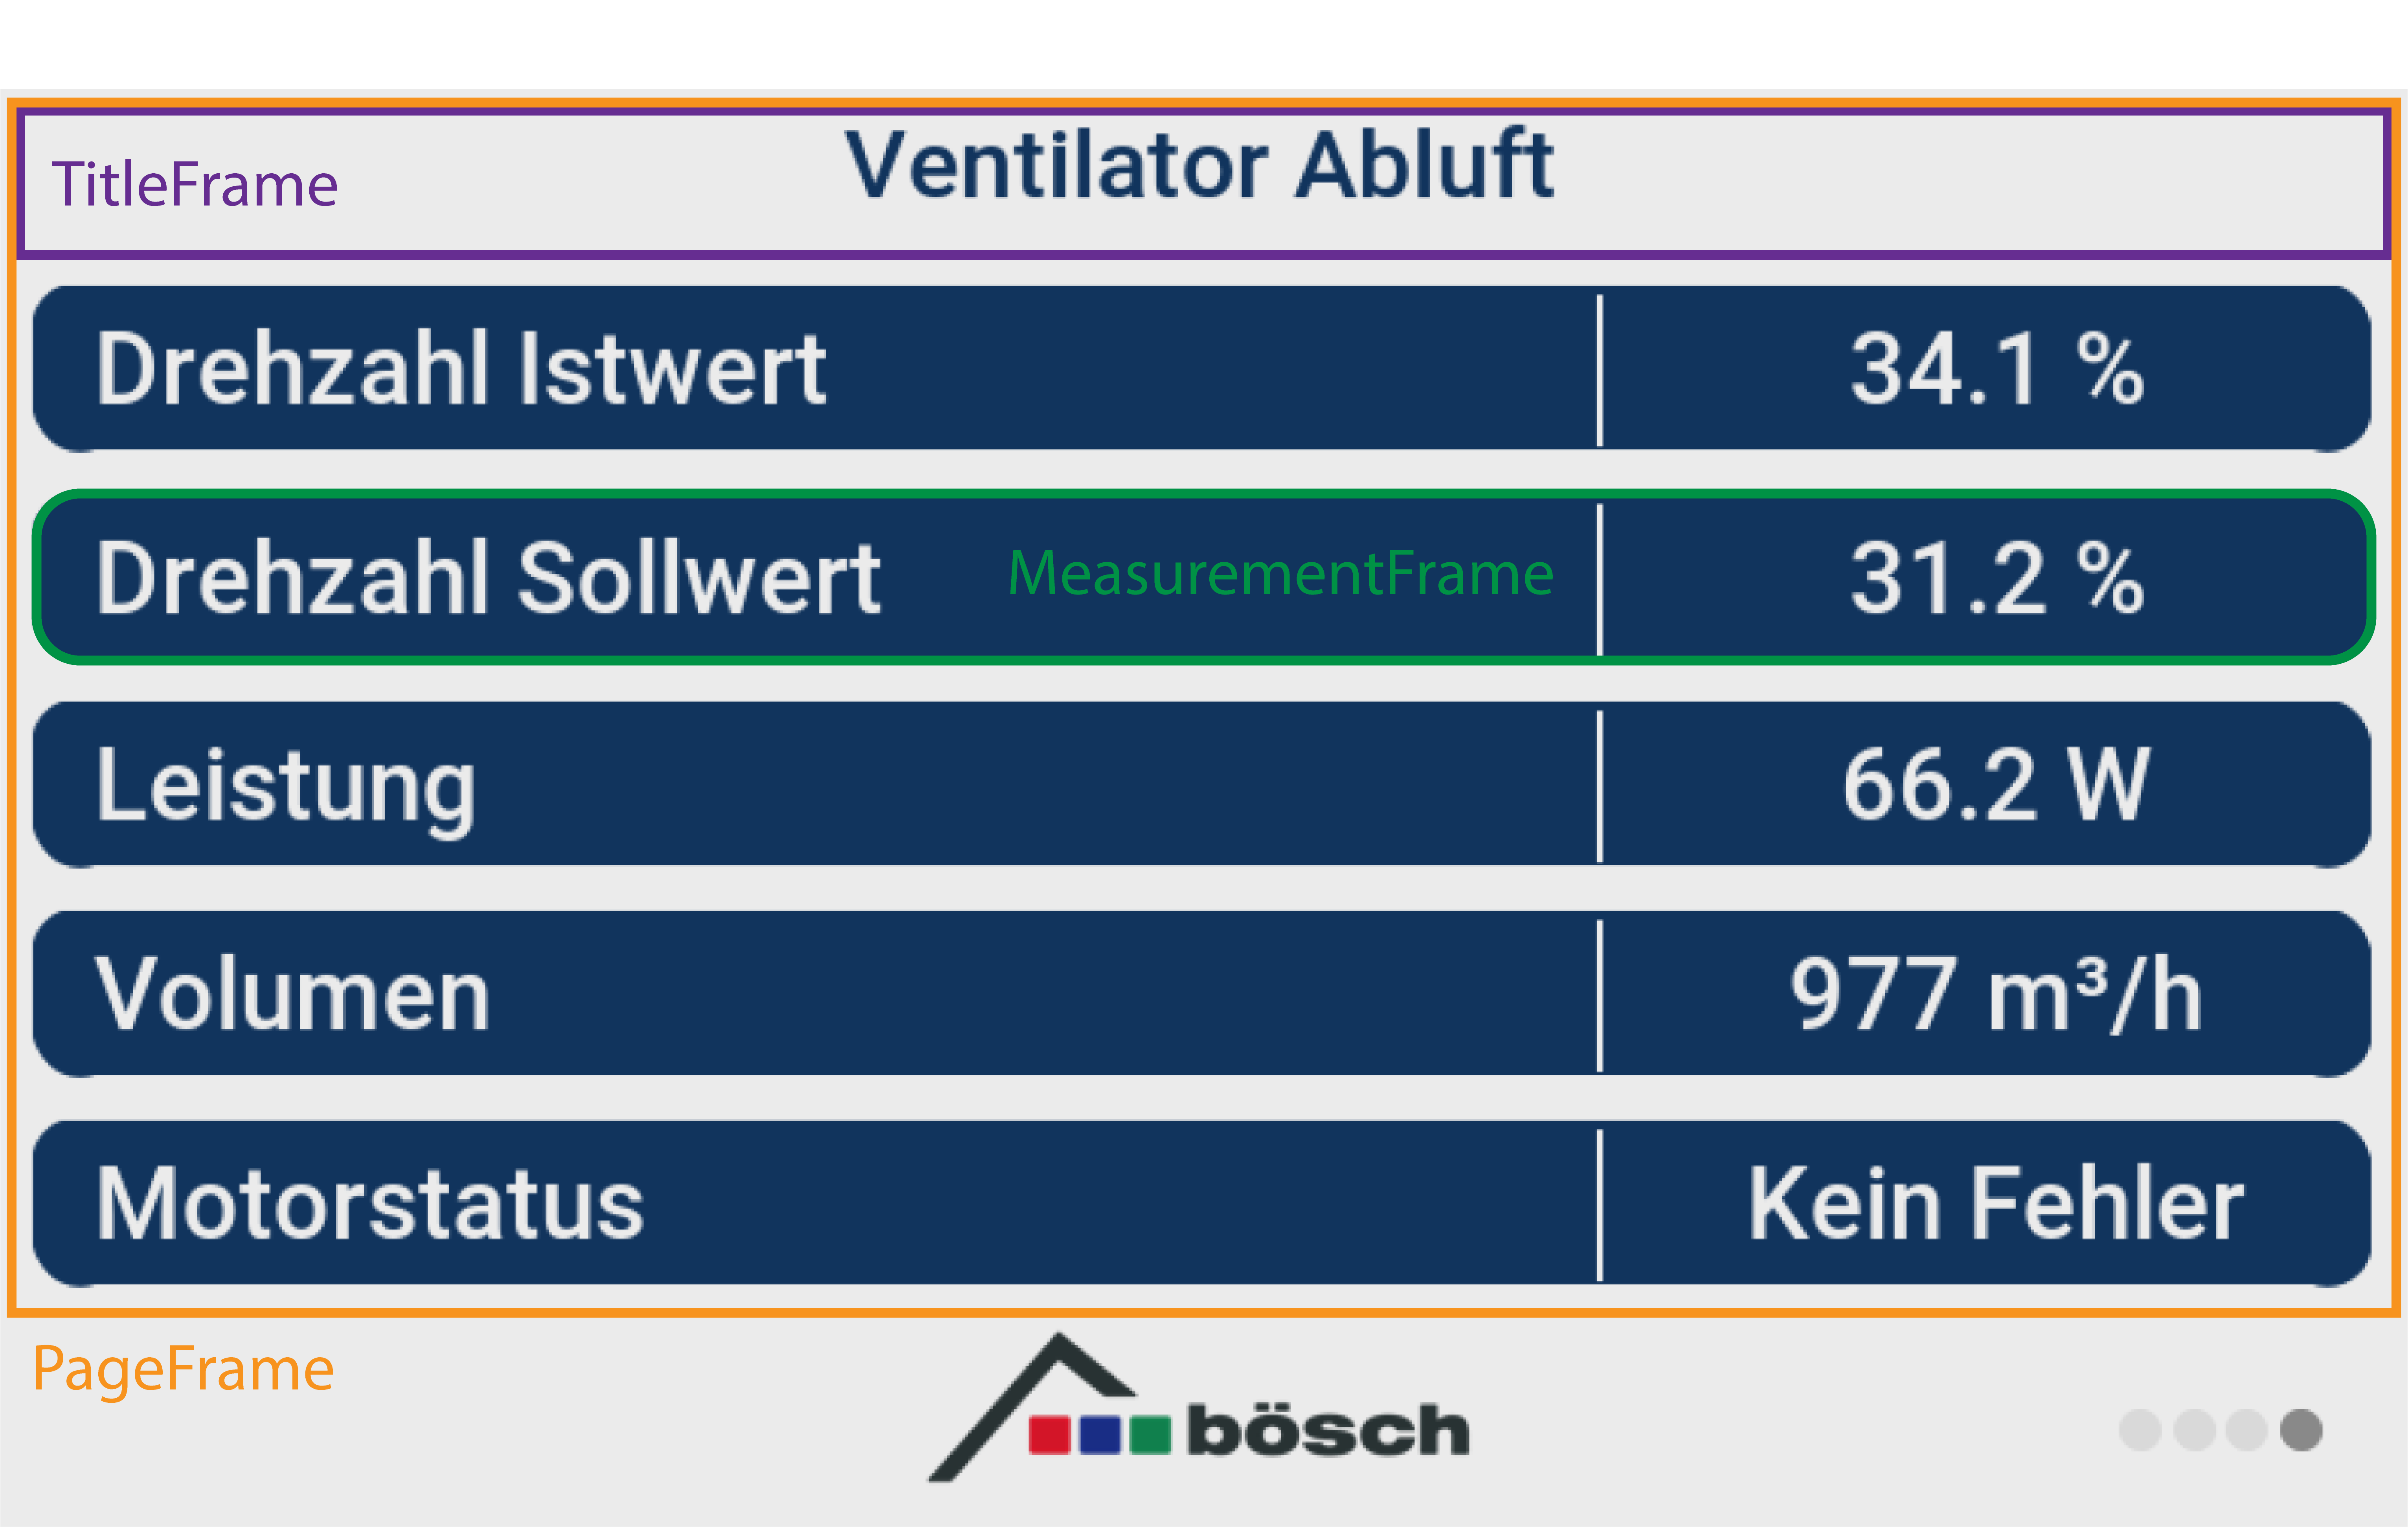
\includegraphics[width=0.90\textwidth]{CTK_components}
	\caption{Ergebnis der \acs{gui} mit Bezeichnungen zugehöriger Klassen \label{fig:ctk_components}}
\end{figure}

\begin{pythoncode}
class MeasurementFrame(ctk.CTkFrame):
	def __init__(self, master, measurement, value, **kwargs):
		super().__init__(master, width=770, height=55, fg_color=title_color, **kwargs)
		
		text_font = ctk.CTkFont(family="Roboto", size=33)
		
		self.measurement_lbl = ctk.CTkLabel(master=self, text=measurement, width=485, height=52, fg_color="transparent", text_color=text_color, anchor=ctk.W, font=text_font)
		self.measurement_lbl.place(relx=0.34, rely=0.5, anchor=ctk.CENTER)
		
		self.value_lbl = ctk.CTkLabel(master=self, text=value, width=190, height=52, fg_color="transparent", text_color=text_color, anchor=ctk.CENTER, font=text_font)
		self.value_lbl.place(relx=0.84, rely=0.5, anchor=ctk.CENTER)
		
		canvas = Canvas(master=self, width=2, height=50, bg=text_color, highlightthickness=0)
		canvas.place(relx=0.67, rely=0.5, anchor=ctk.CENTER)
	
	def set_text(self, measurement, value):
		self.measurement_lbl.configure(text=measurement)
		self.value_lbl.configure(text=value)
\end{pythoncode}
	
\begin{pythoncode}
class PageFrame(ctk.CTkFrame):
	def __init__(self, master, title, parameters, **kwargs):
		super().__init__(master, 800, 515, fg_color="transparent", **kwargs)
		self.measurement_frames = []
		self.title_frame = TitleFrame(master=master, title=title, corner_radius=0)
		
		for parameter in parameters:
			frame = MeasurementFrame(master=master, measurement=parameter.description, value="N/A", corner_radius=15)
			self.measurement_frames.append(frame)
			
	def show_frame(self, show_or_hide):
		if show_or_hide:
			self.title_frame.place(relx=0.5, rely=0.0, anchor=ctk.N)
			self.title_frame.tkraise()
		else:
			self.title_frame.place_forget()
		
		spacing = 0.0
		for my_frame in self.measurement_frames:
			if show_or_hide:
				my_frame.place(relx=0.5, rely=(0.20 + spacing), anchor=ctk.CENTER)
				my_frame.tkraise()
			else:
				my_frame.place_forget()
			spacing += 0.143  # 0.1335
	
	def set_text_at(self, index, measurement, value):
		# ZUM TESTEN, so werden Fehler abgefangen; wird aber eigentlich nicht benötigt!
		if index >= 0 and index < len(self.measurement_frames):
			self.measurement_frames[index].set_text(measurement, value)
\end{pythoncode}


\begin{pythoncode}
class App(ctk.CTk):
	def __init__(self, all_pages, *args, **kwargs):
		super().__init__(*args, **kwargs)
		self.title("Bösch RLT Anzeige")
		self.geometry(f"{app_width}x{app_height}")
		self.attributes('-fullscreen', True)
		self.resizable(False, False)
		self.config(cursor="none")
		
		boesch_logo = ctk.CTkImage(light_image=Image.open("/home/pi/Documents/00_boesch_logo_transparent.png"), dark_image=Image.open("/home/pi/Documents/00_boesch_logo_transparent_dark.png"), size=(230, 230 * (1 / 3)))
		
		self.img_label = ctk.CTkLabel(master=self, image=boesch_logo, text="")
		self.img_label.place(relx=0.5, rely=0.915, anchor=ctk.CENTER)
		
		global page_frame_list
		page_frame_list = []
		global page_indicator_list
		page_indicator_list = []
		
		for page in all_pages:  # Creates Frames based on the sensor data
			page_frame_list.append(PageFrame(master=self, title=page.title, parameters=page.measurements))
		
		print(len(page_frame_list))
		page_frame_list[globals_.current_page].show_frame(True)

		start_x_position = 0.975 - len(page_frame_list) / 45.0
		
		if len(page_frame_list) > 1:
			for i in range(0, len(page_frame_list)):
				page_indicator_list.append(ctk.CTkButton(master=self, width=15, height=15, text="", corner_radius=50, fg_color=("#898989" if i == globals_.current_page else "#D9D9D9")))
				page_indicator_list[i].place(relx=start_x_position + i / 45.0, rely=0.93, anchor=ctk.CENTER)
		
	def set_page_text_at(self, page_index, measurement_index, measurement, value):
		if page_index >= 0 and page_index < len(page_frame_list):
			page_frame_list[page_index].set_text_at(measurement_index, measurement, value)
	
\end{pythoncode}
